\documentclass{article}

\usepackage{fancyhdr}
\cfoot{
\vspace{1mm}\hspace{0.5cm}

\includegraphics[width=0.2\textwidth]{CC-BY-NC-SA.pdf}}

\renewcommand{\headrulewidth}{0pt}
\renewcommand{\footrulewidth}{0pt}
\setlength\headheight{80.0pt}
\addtolength{\textheight}{-80.0pt}

\usepackage[margin = 3cm, footskip = 30pt]{geometry}
\usepackage{amsmath}
\usepackage{blkarray}
\usepackage[table]{xcolor}
\usepackage{amssymb}
\usepackage{amsfonts}

\usepackage{enumerate}
\newcommand\bg{\cellcolor{gray!70}}

\usepackage{stackengine,graphicx}
\def\stacktype{L}
\def\useanchorwidth{T}
\newcommand\strike[1]{\stackon[3.3pt]{#1}{\rule{4.5ex}{1pt}}}
\newcommand\vstrike[1]{\stackon[0pt]{#1}{\smash{\rule[-3pt]{1pt}{2.9ex}}}}
\usepackage{pgfplots}

\pgfplotsset{compat=1.10}
\usepgfplotslibrary{fillbetween}
\usepackage{tikz}
\usetikzlibrary{shapes.geometric, arrows,positioning,automata}
\usepackage{tkz-euclide}
\usetkzobj{all}

\makeatletter
\renewcommand*\env@matrix[1][*\c@MaxMatrixCols c]{
  \hskip -\arraycolsep
  \let\@ifnextchar\new@ifnextchar
  \array{#1}}
\makeatother

\title{Linear Mapping (Part 008)}
\author{Dr Kapil\\kapil $@$ nitkkr $\cdot$ ac $\cdot$ in\\ Department of Computer Applications\\ NIT Kurukshetra}
\date{\today}

\begin{document}
\maketitle
\thispagestyle{fancy}
In the last part, we talked about some basic properties of a vector space spanned by a set of vectors. In this part, we are going to discuss about the vector functions that can translate vectors of a vector space into some other vectors while maintaining their parallelism and even spacing of their grid lines. As a problem solving strategy, it is sometimes easier to solve a similar problem rather than solving a particular problem. And the mapping help us understand the relationship between different vector spaces. Therefore, here we are going to learn about different kind of mappings and their properties.\\

Mapping is another word to refer a function. Now, we want to study those mapping which when used on vectors do not change there property of linearity (the core property). In simpler words, it demands to retain the parallelism and all the grid lines remain evenly spaced (Check 3 Blue 1 Brown Series lecture on linear mapping at https://www.youtube.com/watch?v=kYB8IZa5AuE).\\

Mathematically, if \( \vec{\Phi}: V \rightarrow W \), where $V,~W$ are real vector spaces, then the function $\vec{\Phi}$ is called \textit{linear mapping} if it preserves the structure of the vector space. Formally, $\vec{\Phi}$ should have following properties-
\begin{align}
\Vec{\Phi}(\Vec{x} + \Vec{y}) &= \Vec{\Phi}(\Vec{x}) + \Vec{\Phi}(\Vec{y}) &\forall \Vec{x},\Vec{y} \in V \nonumber \\
\Vec{\Phi}(\lambda \Vec{x}) &= \lambda \Vec{\Phi}(\Vec{x}) &\forall \Vec{x} \in V \text{ and } \forall \lambda \in \mathbb{R} \nonumber
\end{align}

Equivalently, for a vector spaces $V,~W$ a mapping $\vec{\Phi}: V \rightarrow W$ is known as \textit{Linear Mapping} (or \textit{Vector Space homomorphism}  or \textit{Linear Transformation}) if 
\begin{align}
    \forall \Vec{x}, \Vec{y} \in V \text{ and }\forall \lambda , \psi \in \mathbb{R} ~~~~\vec{\Phi} (\lambda \Vec{x} + \psi \Vec{y}) = \lambda \vec{\Phi}(\Vec{x}) + \psi \vec{\Phi}(\Vec{y}) \nonumber
\end{align}

Now, we will see that any linear mapping can be written in the form of matrices. So, first let us check if matrices show linear mapping or not. Or if for any matrix $A$,  $\Vec{x}, \Vec{y} \in \mathbb{R}^n$ then 
\begin{align}
    &A(\Vec{x} + \Vec{y}) = A\Vec{x} + A\Vec{y} &(\text{Matrix multiplication is distributive over vector addition})\nonumber \\
    \text{and } &A(\lambda \Vec{x}) = \lambda A \Vec{x} ~~~~\forall \lambda\in \mathbb{R} &(\text{ Associative Property}) \nonumber
\end{align}

Hence, matrices satisfy both the properties. So, they depict linear mappings. Let us take some examples-\\
\begin{enumerate}
    \item \textbf{Scaling}\\
Let there is mapping that scales an object. So, if there is an object then the mapping will scale it to its twice in such a case if the input vector is \(\begin{pmatrix}  1\\2 \end{pmatrix}\), then the mapped vector will become \(\begin{pmatrix} 2\\4 \end{pmatrix}\) i.e. 
\begin{align}
    \vec{\Phi}(\Vec{u}) &= 2\Vec{u} \nonumber \\
    \vec{\Phi}(\Vec{u} + \Vec{v}) &= 2(\Vec{u} + \Vec{v}) = 2\Vec{u} + 2\Vec{v} = \vec{\Phi}(\Vec{u}) + \vec{\Phi}(\Vec{v}) \nonumber \\
    \vec{\Phi}(\lambda\Vec{u}) &= 2(\lambda\Vec{u}) = \lambda(2\Vec{u}) = \lambda\vec{\Phi}(\Vec{u}) \nonumber
\end{align}
\item \textbf{Rotation}\\
As an another example let us look at mapping that rotates a vector about origin in 2-D
% image need to inserted here
\begin{align}
    \Vec{u} &= \begin{pmatrix}\begin{Vmatrix}\vec{u}\end{Vmatrix}\cos\alpha\\\begin{Vmatrix}\vec{u}\end{Vmatrix}\sin\alpha\end{pmatrix} = \begin{pmatrix}x\\y\end{pmatrix} \nonumber \\
    \Vec{v} &= \begin{pmatrix}\begin{Vmatrix}\Vec{v}\end{Vmatrix}\cos\beta\\\begin{Vmatrix}\Vec{v}\end{Vmatrix}\sin\beta\end{pmatrix} = \begin{pmatrix}x_n\\y_n\end{pmatrix} \nonumber
\end{align}
as magnitude is same for the rotated vectors \(\begin{Vmatrix}\Vec{u}\end{Vmatrix} = \begin{Vmatrix}\Vec{v}\end{Vmatrix} = r=\sqrt{x^2+y^2}=\sqrt{x_n^2+y_n^2}\). Also, \(x=r\cos\alpha,~~y=r\sin\alpha.\) \\
\begin{tikzpicture}
\draw[help lines] (0,0) grid (5,5);
\draw[->,thick] (0,0) -- (6,0);
\draw[->,thick] (0,0) -- (0,6);
\draw[->,thick] (0,0) -- ++(30:4cm) node[pos=1.5]{Original ($\Vec{u}$\\)};
\draw [red,->,thick] (0,0) -- ++(60:4cm) node[above]{Rotated ($\Vec{v}$\\)};
  \tkzDefPoint(0,0){O}
\tkzDefPoint(0:1){Aalpha} 
\tkzDefPoint(30:1){Balpha}
\tkzDefPoint(0:1.5){Abeta} 
\tkzDefPoint(60:1.5){Cbeta}
\tkzDefPoint(30:2){Btheta} 
\tkzDefPoint(60:2){Ctheta}

\tkzDrawArc[->,thick,color=blue](O,Aalpha)(Balpha) \tkzDrawArc[->,thick,color=purple](O,Abeta)(Cbeta) 
\tkzDrawArc[->,thick,color=green](O,Btheta)(Ctheta) 
%https://tex.stackexchange.com/questions/66216/draw-arc-in-tikz-when-center-of-circle-is-specified/66219
\tkzLabelAngle[dist=1.3,color=blue](Aalpha,O,Balpha){$\alpha$}
\tkzLabelAngle[dist=1.8,color=purple](Abeta,O,Cbeta){$\beta$}
\tkzLabelAngle[dist=2.3,color=green](Btheta,O,Ctheta){$\theta$} % https://tex.stackexchange.com/questions/521328/unit-circle-and-circle-of-radius-r
\end{tikzpicture}

\begin{align*}
{x_n} &= r\cos{\beta}=r\cos{(\alpha+\theta)}\\
&= r[\cos{\alpha}\cos{\theta}-\sin{\alpha}\sin{\theta}]\\
&= x\cos{\theta}-y\sin{\theta}\\
{y_n} &= r\sin{\beta} = r\sin{(\alpha+\theta)}\\
&= r[\sin{\alpha}\cos{\theta}+\cos{\alpha}\sin{\theta}]\\
&= y\cos{\theta}+x\sin{\theta}\\
\end{align*}
\begin{align*}
\because \vec{\phi}
\left(\begin{pmatrix}
 x\\y
\end{pmatrix}
\right)&=\begin{pmatrix} 
\phi_1(x,y)\\ \phi_2(x,y)
\end{pmatrix}
=\begin{pmatrix}
 x\cos\theta-y\sin{\theta}\\x\sin\theta+y\cos{\theta}
\end{pmatrix}
\\
\vec{\phi} (\Vec{u}+\Vec{v}) &=\vec{\phi}
\bigg(\begin{pmatrix}
 {x_1}+{x_2}\\
 {y_1}+{y_2}
\end{pmatrix}\bigg)
=\begin{pmatrix}
 ({x_1}+{x_2})\cos{\theta}-({y_1}+{y_2})\sin{\theta}\\
 ({x_1}+{x_2})\sin{\theta}+({y_1}+{y_2})\cos{\theta}
\end{pmatrix}
\\
&=\begin{pmatrix}
 {x_1}\cos{\theta}+{x_2}\cos{\theta}-y_1\sin{\theta}-{y_2}\sin{\theta}\\
 {x_1}\sin{\theta}+{x_2}\sin{\theta}+y_1\cos{\theta}+{y_2}\cos{\theta}
 \end{pmatrix}
 \\
 &=\begin{pmatrix}
 {x_1}\cos{\theta}-{y_1}\sin{\theta}\\{x_1}\sin{\theta}+{y_1}\cos{\theta}
\end{pmatrix}+
\begin{pmatrix}
 {x_2}\cos{\theta}-{y_2}\sin{\theta}\\{x_2}\sin\theta+y_2\cos{\theta}
\end{pmatrix}\\
 &=\vec{\phi}(\Vec{u})+\vec{\phi}(\Vec{v})
 \end{align*}
Thus, \(\vec{\phi}(\Vec{u}+\Vec{v}) = \vec{\phi}
\left(\begin{pmatrix}
 {x_1}\\{y_1}
\end{pmatrix}
\right) +
\vec{\phi}
\left(\begin{pmatrix}
 {x_2}\\{y_2}
\end{pmatrix}
\right)\), here we have assumed \(\Vec{u}=\begin{pmatrix}
 {x_1}\\{y_1}
\end{pmatrix} \text{ and } \Vec{v}=\begin{pmatrix}
 {x_2}\\{y_2}
\end{pmatrix}\).\par
Further,
\begin{align*}
 \vec{\phi}(\lambda\Vec{u})=\vec{\phi}\left(\begin{pmatrix}
 \lambda x\\ \lambda y
\end{pmatrix}
 \right)&=
 \begin{pmatrix}
 \lambda x\cos\theta-\lambda y\sin{\theta}\\\lambda x\sin\theta+\lambda y\cos{\theta}\end{pmatrix}
\\
 &= \lambda\begin{pmatrix}
 x\cos\theta-y\sin{\theta}\\x\sin\theta+y\cos{\theta}
\end{pmatrix}\\
\therefore \vec{\phi}(\lambda\Vec{u}) &= \lambda\vec{\phi}(\Vec{u})
\end{align*}
\end{enumerate}

Therefore, you can see that rotation and scaling operations are linear mapping for 2-D vectors. Now, let us see some rules of differentiation.\\

Let $f(\cdot) \text{ and } g(\cdot) \text{ are two functions and }\phi\text{ is mapping defined on set of functions such that } \phi(f(x))=\frac{d}{dx}f(x)$, then 
\begin{align*}
    \phi(f(x)+g(x))&=\frac{d}{dx}(f(x)+g(x))\\
    &=\frac{d}{dx}f(x)+\frac{d}{dx}g(x)\\
    &=\phi (f(x))+\phi(g(x)).
\end{align*}
Also, 
\begin{align*}
    \phi(\lambda f(x))&=\frac{d}{dx}(\lambda f(x))\\
    &=\lambda\frac{d}{dx}f(x)\\
    &=\lambda \phi (f(x))
\end{align*}

So a lot of operations are linear mappings. And studying them will help dealing with them programmatic-ally. Soon, we will see that finding derivatives can be automatic. \par

Let us take another example. Let $f(x,y,z)=(2x+3y,x+y-3z,2z)$ be multi-valued function. That is $f:\mathbb{R}^3\rightarrow\mathbb{R}^3$. This we can assume as a functions that takes a vector of $\mathbb{R}^3$ as input and generates another vector as output of $\mathbb{R}^3$.
\[
\vec{f}\left(\begin{pmatrix}
x\\y\\z
\end{pmatrix}\right)=
\begin{pmatrix}
2x + 3y\\
x + y + 3z\\
2z
\end{pmatrix}
\hspace{3mm}
\forall x, y, z \in \mathbb{R}
\]
\\
Now, prove if it is a linear mapping.\\\\
\textbf{Proof:}
\[
\text{Let } \Vec{u},\Vec{v} \in \mathbb{R}^3, \Vec{u} =
\begin{pmatrix}
u_1\\u_2\\u_3
\end{pmatrix},
\Vec{v}=
\begin{pmatrix}
 v_1\\v_2\\v_3
\end{pmatrix}
\text{ then, }
\]

\begin{align*}
\vec{f}\begin{pmatrix}
 \Vec{u}+\Vec{v}
\end{pmatrix} &=
\vec{f}\left(\begin{pmatrix}
 u_1 + v_1\\
 u_2 + v_2\\
 u_3 + v_3
\end{pmatrix}\right) &=
\begin{pmatrix}
 2(u_1 + v_1) + 3(u_2 + v_2)\\
 (u_1 + v_1) + (u_2 + v_2) - 3(u_3 + v_3)\\
 2(u_3 + v_3)
\end{pmatrix}\\
&= \begin{pmatrix}
(2u_1 + 3u_2) + (2v_1 + 3v_2)\\
(u_1 + u_2 - 3u_3) + (v_1 + v_2 - 3v_3)\\
2u_3 + 2v_3
\end{pmatrix} &= \begin{pmatrix}
2u_1 + 3u_2\\
u_1 + u_2 - 3u_3\\
2u_3 
\end{pmatrix}+\begin{pmatrix}
2v_1 + 3v_2\\
v_1 + v_2 - 3v_3\\
2v_3
\end{pmatrix}\\
&= \vec{f}(\Vec{u}) + \vec{f}(\Vec{v}).
\end{align*}

Similarly, you can prove 
\[
\vec{f}(c\Vec{u}) = 
\vec{f}\left(\begin{pmatrix}
cu_1\\
cu_2\\
cu_3
\end{pmatrix}\right)=
\begin{pmatrix}
 2cu_1 + 3cu_2\\
 cu_1 + cu_2 - 3cu_3\\
 2cu_3
\end{pmatrix}=
c\begin{pmatrix}
 2u_1 + 3u_2\\
 u_1 + u_2 - 3u_3\\
 2u_3
\end{pmatrix}=
c\vec{f}(\Vec{u})
\]

\textbf{Definition}\\
Consider a mapping $\vec{\phi} \colon \mathbb{V} \longrightarrow \mathbb{W}$ where, $\mathbb{V},\mathbb{W}$ are arbitrary sets of vectors. then $\vec{\phi}$ is called\\
\begin{enumerate}[i.]
    \item \textit{Injective} if $(\forall \Vec{x},\Vec{y} \in \mathbb{V})\colon \vec{\phi}(\Vec{x})= \vec{\phi}(\Vec{y})\implies \Vec{x} = \Vec{y}$   (One-One)
    \item \textit{Surjective} if $\vec{\phi}(\mathbb{V}) = \mathbb{W}$ i.e. each element of $\mathbb{W}$ has some pre-image in $\mathbb{V}$     (Onto)
    \item \textit{Bijective} if it is One-One and Onto both.
\end{enumerate}

A bijective mapping can be undone, that is if $\vec{\phi}$ is bijective, then $\exists~\vec{\psi}\colon \mathbb{W}\longrightarrow\mathbb{V}$ such that $(\vec{\psi} \circ \vec{\phi})(\Vec{x}) = \vec{x}$. The function $\vec{\psi}$ is said to be inverse of $\vec{\phi}$ and usually denoted as $\vec{\phi}^{-1}$.\\

There are some special mappings-
\begin{enumerate}[i.]
    \item Isomorphism: $\vec{\phi}\colon\mathbb{V}\longrightarrow\mathbb{W}$  linear and bijective
    \item Endomorphism: $\vec{\phi}\colon\mathbb{V}\longrightarrow\mathbb{V}$  linear
    \item Automorphism: $\vec{\phi}\colon\mathbb{V}\longrightarrow\mathbb{V}$  linear and bijective\\
    id: $\vec{\phi}\colon\mathbb{V}\longrightarrow\mathbb{V}, \Vec{x}\longrightarrow\Vec{x}$ as identity mapping or identity automorphism. 
\end{enumerate}

Therefore, finite dimensional vector space $\mathbb{V}$ and $\mathbb{W}$ are isomorphic if and only if $\dim(\mathbb{V}) = \dim(\mathbb{W})$\\
This means that vector spaces of same dimension are kind of same thing as they can be transformed among each other without incurring any loss or increment.\\
\textbf{Example}\\
Usage of above theorem- Vector space of $\mathbb{R}^{m\times n}$ rectangular matrices can be treated as vector space with $m\times n$ dimension. As there exists a linear bijective mapping that transforms one onto other.
\begin{itemize}
    \item if $\vec{\phi}\colon \mathbb{V}\longrightarrow\mathbb{W}$ and $\vec{\psi}\colon \mathbb{W}\longrightarrow\mathbb{X}$ are linear mapping then $\vec{\psi}\circ\vec{\phi}\colon \mathbb{V}\longrightarrow\mathbb{X}$ is also linear mapping.
    \item if $\vec{\phi}\colon \mathbb{V}\longrightarrow\mathbb{W}$ is a linear and bijective mapping(isomorphism), then $\vec{\phi} ^{-1}\colon \mathbb{W}\longrightarrow \mathbb{V}$ is also an isomorphism.
    \item You must be able to recall the fact that a function has its inverse as a function iff it is bijective.
\end{itemize}
Let us take some examples to understand the above concepts. Consider the below function-
\[y = f(x) = x^2  ~~~ f\colon\mathbb{R}\longrightarrow\mathbb{R}\]
For it to be bijective function, both Figures (\ref{fig:sqr} and \ref{fig:sqrt}) should depict functions.
\begin{figure}
    \centering
\begin{tikzpicture}
\begin{axis}[grid=both, restrict x to domain=-3:3, restrict y to domain=-1:9,xtick distance=1,ytick distance=1,axis lines = middle, xlabel=$x$, ylabel=$y$, label style = {at={(ticklabel cs:1.1)}}]    
    \addplot [name path=plot1, ultra thin, domain=-3:3, samples=100]{x^2};
\end{axis}
\end{tikzpicture}
\caption{$y=x^2$} \label{fig:sqr}
\end{figure}

\begin{figure}
    \centering
\begin{tikzpicture}
\begin{axis}[grid=both,restrict x to domain=-1:9, restrict y to domain=-3:3, xtick distance=1,ytick distance=1,axis lines = middle,xlabel=$x$,ylabel=$y$,label style =
               {at={(ticklabel cs:1.1)}}]
               
    \addplot [ultra thin, domain=0:10, samples=121]{x^0.5};
    \addplot [ultra thin, domain=0:10, samples=121]{-x^0.5};
    
\end{axis}
\end{tikzpicture}
\caption{$y^2=x$}
    \label{fig:sqrt}
\end{figure}

Above stated (Figure \ref{fig:sqr}) is a function. But there are two problems for Figure (\ref{fig:sqrt}) to be a function-
\begin{enumerate}
    \item for every non-negative value of $x$ ($x\geq 0$), there are two images, which can be obvious by taking a vertical line and looking number of intersection, for a function it should intersect exactly once. While here it is intersecting twice when $x\geq 0$. Alternatively, a horizontal line above $x$-axis cuts the graph in two places, making the original function \textit{Many-one} (and not (\textit{One-One}).
    
    \item Further, for negative values of $x$, Figure (\ref{fig:sqrt}) there is no mapping, which can be visible in the original function by taking horizontal line below $x$-axis and it does not cut the graph anywhere. Thereby making Figure (\ref{fig:sqr}) \textit{into} function, that is at least for some $y$ it may not have pre-image back in the  domain. 
\end{enumerate}
So, a graphical test for a function is that any vertical line should intersect exactly at once with the graph. For one-one, any horizontal line should not cut more than once. And if the function is onto the horizontal line should cut the graph at least once. Thus for a bijective function (one-one and onto) every horizontal line in co-domain should cut the graph exactly once.\\

Thus, if we change $f$ (Figure \ref{fig:sqr}) to-
\begin{enumerate}
    \item \(g\colon\mathbb{R}\longrightarrow\mathbb{R}^+\cup\{0\} \text{makes it onto.}\) 
    \item $h\colon \mathbb{R}^+ \cup \{0\} \longrightarrow\mathbb{R}$ make it one-one. 
\end{enumerate}

Therefore, for the example we have to accommodate both the changes. So the bijective function may be-\\
$y = f(x) = x^2~~~~f\colon\mathbb{R}^+\cup\{0\}\longrightarrow\mathbb{R}^+\cup\{0\}$.\\

In the next lecture, we are going to learn about matrix representation of linear mappings. One step closer to automating large number of mappings including derivatives.
\end{document}